
% ----------------------------------------------------------------------
%  Set the document class
% ----------------------------------------------------------------------
\documentclass[11pt,a4paper,twoside]{article}

% ----------------------------------------------------------------------
% Define external packages, language, margins, fonts and new commands
% ----------------------------------------------------------------------
%\input{preamble} 
\usepackage[utf8]{inputenc}   % <<<<< Linux
\usepackage[english]{babel} % <<<<< English
\usepackage{notoccite}
\usepackage[skip=0.5\baselineskip]{caption}
\hyphenation{GTKWave}
\usepackage{listings}
\usepackage[all]{nowidow}

%blind text
%\usepackage{lipsum}

\usepackage{graphicx}
\graphicspath{ {./} {../../figlib/} }
\def\FontLn{% 16 pt normal
  \usefont{T1}{phv}{m}{n}\fontsize{16pt}{16pt}\selectfont}
\def\FontLb{% 16 pt bold
  \usefont{T1}{phv}{b}{n}\fontsize{16pt}{16pt}\selectfont}
\def\FontMn{% 14 pt normal
  \usefont{T1}{phv}{m}{n}\fontsize{14pt}{14pt}\selectfont}
\def\FontMb{% 14 pt bold
  \usefont{T1}{phv}{b}{n}\fontsize{14pt}{14pt}\selectfont}
\def\FontSn{% 12 pt normal
  \usefont{T1}{phv}{m}{n}\fontsize{12pt}{12pt}\selectfont}

% Use Arial font as default
%
\renewcommand{\rmdefault}{phv}
\renewcommand{\sfdefault}{phv}
\usepackage{geometry}	
\geometry{verbose,tmargin=2.5cm,bmargin=2.5cm,lmargin=2.5cm,rmargin=2.5cm}

%\usepackage{setspace}
%\renewcommand{\baselinestretch}{1.5}

\usepackage[pdftex]{hyperref} % enhance documents that are to be
                              % output as HTML and PDF
\hypersetup{colorlinks,       % color text of links and anchors,
                              % eliminates borders around links
%            linkcolor=red,    % color for normal internal links
            linkcolor=black,  % color for normal internal links
            anchorcolor=black,% color for anchor text
%            citecolor=green,  % color for bibliographical citations
            citecolor=black,  % color for bibliographical citations
%            filecolor=magenta,% color for URLs which open local files
            filecolor=black,  % color for URLs which open local files
%            menucolor=red,    % color for Acrobat menu items
            menucolor=black,  % color for Acrobat menu items
%            pagecolor=red,    % color for links to other pages
            pagecolor=black,  % color for links to other pages
%            urlcolor=cyan,    % color for linked URLs
            urlcolor=black,   % color for linked URLs
	          bookmarks=true,         % create PDF bookmarks
	          bookmarksopen=false,    % don't expand bookmarks
	          bookmarksnumbered=true, % number bookmarks
	          pdftitle={report},
            pdfauthor={Andre C. Marta},
%            pdfsubject={Thesis Title},
%            pdfkeywords={Thesis Keywords},
            pdfstartview=FitV,
            pdfdisplaydoctitle=true}

\usepackage[numbers,sort&compress]{natbib} % <<<<< References in numbered list [1],[2],...
\usepackage{subcaption} 
\usepackage{mdframed}

%%%%%%%%%%%%%%%%%%%%%%%%%%%%%%%%%%%%%%%%%%%%%%%%%%%%%%%%%%%%%%%%%%%%%%%%
%     Begin Document                                                   %
%%%%%%%%%%%%%%%%%%%%%%%%%%%%%%%%%%%%%%%%%%%%%%%%%%%%%%%%%%%%%%%%%%%%%%%%


\begin{document}

% Set plain page style (no headers, footer with centered page number)
\pagestyle{plain}

% Set roman numbering (i,ii,...) before the start of chapters
%\pagenumbering{roman}

% ----------------------------------------------------------------------
%  Cover page
% ----------------------------------------------------------------------
%%%%%%%%%%%%%%%%%%%%%%%%%%%%%%%%%%%%%%%%%%%%%%%%%%%%%%%%%%%%%%%%%%%%%%%%
%                                                                      %
%     File: Thesis_FrontCover.tex                                      %
%     Tex Master: Thesis.tex                                           %
%                                                                      %
%     Author: Andre C. Marta                                           %
%     Last modified :  2 Jul 2015                                      %
%                                                                      %
%%%%%%%%%%%%%%%%%%%%%%%%%%%%%%%%%%%%%%%%%%%%%%%%%%%%%%%%%%%%%%%%%%%%%%%%

\thispagestyle {empty}

% IST Logo - Signature A
% parameters: bb=llx lly urx ury (bounding box), width=h_length, height=v_length, angle=angle, scale=factor, clip=true/false, draft=true/false. 
\includegraphics[bb=9.5cm 11cm 0cm 0cm,scale=0.29]{IST_A_CMYK_POS}

\begin{center}
%
% Figure (Image or plot)
\vspace{1.0cm}
% height = 50 mm
%\includegraphics[height=50mm]{Figures/Airbus_A350.jpg}

% Title, author and degree
\vspace{1cm}
{\FontLb Circuit Theory and Electronics Fundamentals} \\ % <<<<< EDIT TITLE
\vspace{5cm}
{\FontLn T2 Laboratory Report}\vspace{1cm} \\
\vspace{5cm}
{\FontLb Group 34} \\
\vspace{1cm}
{\FontSn José Bento, Nº 95815} \\
{\FontSn Thomas Childs, Nº 95847} \\
{\FontSn Luís Pacheco, Nº 96425} \\
\vspace{1cm}
{\FontSn Aerospace Engineering (MEAer), Técnico, University of Lisbon} \\ % <<<<< EDIT COURSE
\vspace{1cm}
{\FontSn April 5, 2021} \\ % <<<<< EDIT DATE (corresponds to date of oral examination)
%
\end{center}




% ----------------------------------------------------------------------
% Dedication page (optional)
% ----------------------------------------------------------------------
%\input{dedication} 
%\cleardoublepage

% ----------------------------------------------------------------------
%  Acknowledgments (optional)
% ----------------------------------------------------------------------
%\input{acknowledgements}
%\cleardoublepage

% ----------------------------------------------------------------------
%  Abstract (both in English and Portuguese)
% ----------------------------------------------------------------------
%\input{resumo} 
%\cleardoublepage

%\input{abstract} 

% ----------------------------------------------------------------------
%  Table of contents, list of tables, list of figures and nomenclature
% ----------------------------------------------------------------------

% Table of contents
\pagebreak
\tableofcontents
\vspace{18cm}
\pagebreak
% List of tables
%\addcontentsline{toc}{section}{\listtablename}
%\listoftables
%\cleardoublepage 

% List of figures
%\addcontentsline{toc}{section}{\listfigurename}
%\listoffigures
%\cleardoublepage 

% Set arabic numbering (1,2,...) after preface
%
%\setcounter{page}{1}
%\pagenumbering{arabic}

% ----------------------------------------------------------------------
%  Body
% ----------------------------------------------------------------------
\pagebreak
\section{Introduction}
\label{sec:introduction}
% state the learning objective

\par The objective of this laboratory assignment is to study a circuit containing independent and 
linearly dependent voltage and current sources. The circuit also contains 7 resistors, totaling 11 components.\par
The circuit has 8 nodes and 4 meshes. The nodes of the circuit were numbered arbitrarily (from {\it$V_{0}$}  to {\it$V_{7}$} ), and it was considered that {\it node 0} was the ground node. The voltage-controlled current source {\it $I_b$} has a linear dependence on Voltage {\it $V_b$}, of constant {\it $K_b$}. The voltage {\it $V_b$} is the voltage drop at the ends of resistor {\it $R_3$}. The current-controlled voltage source {\it $V_c$} has a linear dependece on current {\it $I_c$}, of constant {\it $K_c$}. The control current {\it $I_c$} is the current that passes through the resistor {\it $R_6$}.
The circuit can be seen in \textbf{Figure~\ref{fig:circuit_t1}}.\par
The values for the resistors, the independent sources and the  constants for the dependent 
sources are presented in \textbf{Table~\ref{tab:python_values}}. These values were obtained using the
Python script provided by the Professor responsable for the laboratory assigment
and using the number 95815 as the seed.\par

In Section~\ref{sec:analysis}, a theoretical analysis of the circuit is
presented using two methods: the mesh analysis and the nodal analysis. In Section~\ref{sec:simulation}, the circuit is analysed by
simulation using the program Ngspice, and the results are compared to the theoretical results obtained in
Section~\ref{sec:analysis}. The conclusions of this study are outlined in
Section~\ref{sec:conclusion}.

\begin{figure}[h] \centering
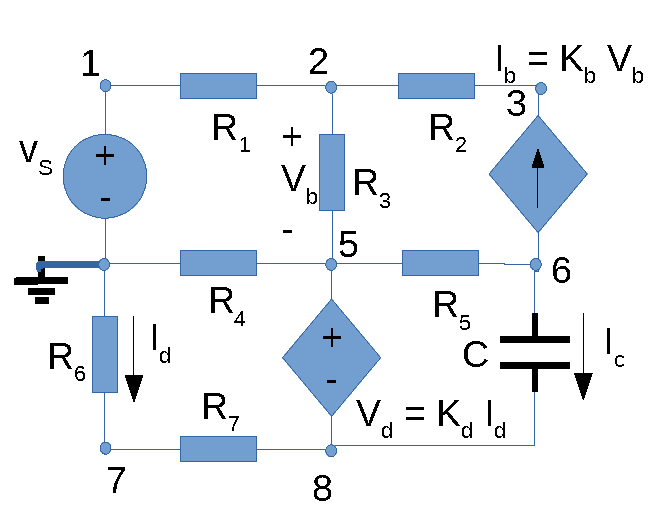
\includegraphics[width=0.9\linewidth]{circuit_t1.pdf}
\caption{Circuit in study}
\label{fig:circuit_t1}
\end{figure}


\begin{table}[h]
  \centering
  \begin{tabular}{|l|r|}
    \hline    
    {\bf Name} & {\bf Python-generated values} \\ \hline
	R1 &  1.04606282456 \\ \hline
	R2 &  2.00732621328 \\ \hline
	R3 &  3.06060705885 \\ \hline
	R4 &  4.07055531265 \\ \hline
	R5 &  3.1225213804 \\ \hline
	R6 &  2.06927045958 \\ \hline
	R7 &  1.01531018068 \\ \hline
	Va &  5.24359648479 \\ \hline
	Id &  1.01891541651 \\ \hline
	Kb &  7.0473187437 \\ \hline
	Kc &  8.3479788681 \\ 
	\hline

  \end{tabular}
  \caption{The variables that start with an {\it R} are the values of the resistors 
    and are expressed in  kiloohm  (kOhm); the variable {\it Va} is a {\it voltage} and is expressed in
    Volt (V) and the variable {\it Id}  is a {\it current} and expressed in
   miliAmpere (mA). The constants {\it Kc} and {\it Kb} are  expressed in
   kiloOhm  (kOhm) and miliSiemens (mS), respectively.}
  \label{tab:python_values}
\end{table}






\section{Theoretical Analysis}
\label{sec:analysis}

In this section, the circuit shown in Figure~\ref{fig:circuit_t1} is analysed
theoretically, in terms of its time and frequency responses.

\section{Time response}

The circuit consists of a single V-R-C loop where a current $i(t)$ circulates. The
voltage source $v_I(t)$ drives its input, and the output voltage $v_O(t)$ is taken from
the capacitor terminals. Applying the Kirchhoff Voltage Law (KVL), a single
equation for the single loop in the circuit can be written as

\begin{equation}
  Ri(t) + v_O(t) = v_I(t).
  \label{eq:kvl}
\end{equation}

Because $v_O$ is the voltage between capacitor C's plates, it is related to the
current $i$ by
\begin{equation}
  i(t) = C\frac{dv_O}{dt}.
\end{equation}

Hence, Equation~(\ref{eq:kvl}) can be rewritten as
\begin{equation}
  RC\frac{dv_O}{dt} + v_O(t) = v_I.
  \label{eq:kvl2}
\end{equation}

Equation~(\ref{eq:kvl2}) is a linear differencial equation whose solution is a
superposition of a natural solution $v_{On}$ and a forced solution $v_{Of}$:

\begin{equation}
  v_O(t) = v_{On}(t) + v_{Of}(t).
  \label{eq:vo_sol}
\end{equation}

As learned in the theory classes the natural solution is of the form
\begin{equation}
  v_{On}(t) = Ae^{-\frac{t}{RC}},
  \label{eq:vo_nat}
\end{equation}
where $A$ is an integration constant.

The forced solution is of the form given in Equation~(\ref{eq:vo_for}) and is
illustrated in Figure~\ref{fig:forced}.

\begin{equation}
  V_{Of}(t) = |\bar{V}_{Of}| cos(\omega t + \angle \bar{V}_{Of}),
  \label{eq:vo_for}
\end{equation}


%\begin{figure}[h] \centering
%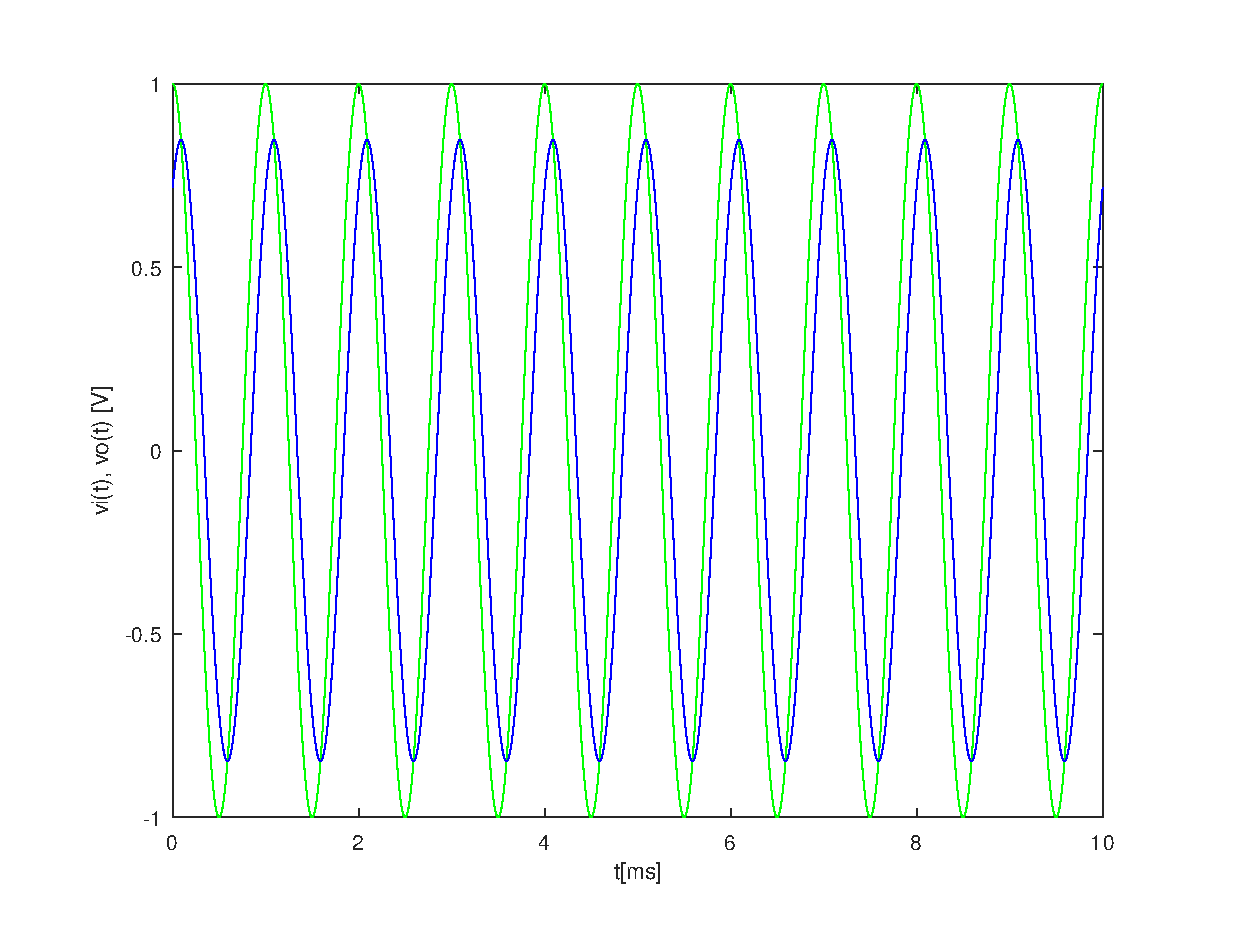
\includegraphics[width=0.8\linewidth]{forced.eps}
%\caption{Forced sinusoidal response.}
%\label{fig:forced}
%\end{figure}

\section{Frequency response}


\section{Simulation Analysis}
\label{sec:simulation}

The main circuit used to simulate the output impedance of the amplifier as a whole was the one that can be found in the following figure (repeteated from the analysis section).

\begin{figure}[h] \centering
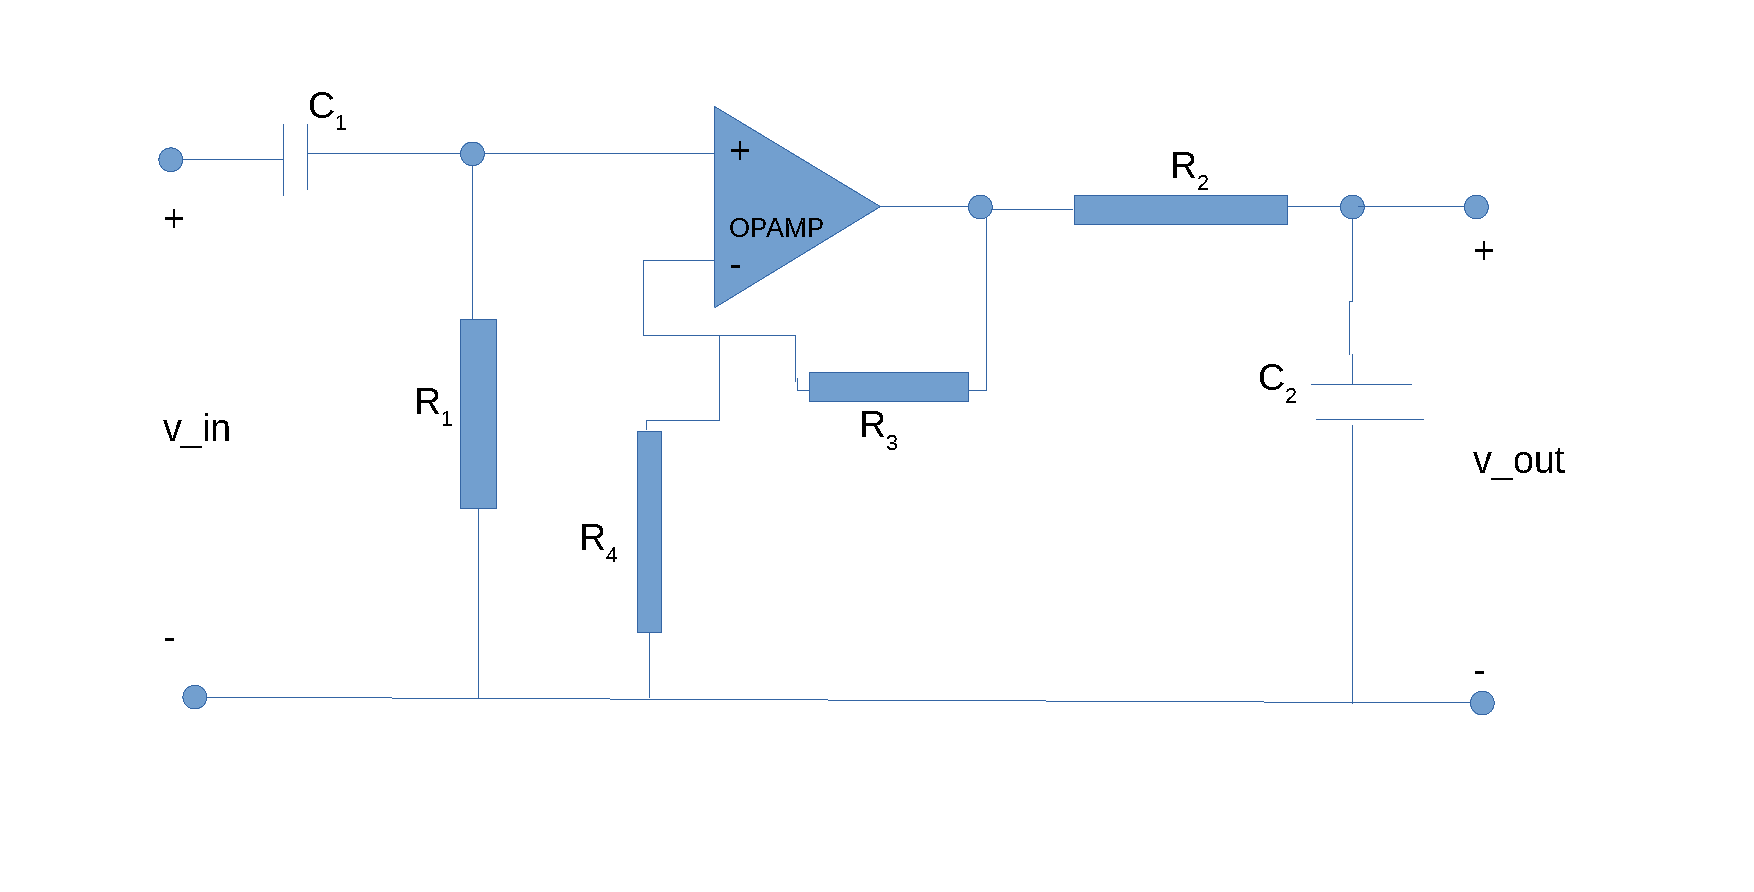
\includegraphics[width=0.95\linewidth]{diagram_t5.pdf}
%\vspace{-7cm}
\caption{Diagram of the circuit considered for the computations and simulations.}
\label{fig:diagram_t5_2}
\end{figure}


Initially, we began by translating this circuit to the Ngspice language, and ensuring the simulation was running smoothly, with random values for the parameters. Next, we automated the merit computation, and ensured all the correct plots were being adequately printed. Only then did we use the formulas referred to in the previous section, to try to work out a solution that gave us the desired pass band (at 1kHz), as well as the desired (40dB) gain. However, this was relatively easy, as the presential lab sesson had been quite informative and there we had already arrived at a setup that seemed to ensure us, approximately, the desired results. More on this in the following section.

However, we soon realized that the theoretical model we were based on was quite far from the simulation results... Having read up on the online class forum and thought about the problem at hand, we realized that this was mainly due to the way we were calculating the cutoff frequencies and the fact that the OPAMP model used was way more complex: besides being far from the ideal OPAMP model considered in our computations, the presence of capacitors (and not insignificant ones, at that!) had an impact on these same cutoff frequencies. As the objective all along was to maximize the Ngspice merit, and not the theoretical one, we focussed on improving this figure. This led us to opting for what might seem like strange combinations, that would never work on paper, but that did in practice. This process was quite iterative, due to a solid grasp on the concept of cutoff frquencies and how they should be altered by the variation of the corresponding resistor or capacitor, we managed to achieve a relatively central frquency at 1kHz. The gain was easier to fine-tune, with a relatively simple expression $1+\frac{R_3}{R_4}$ (this is just the gain from the OPAMP, not yet affected by the voltage drop across the input and output filters); here the limiting factor really was the limitation in terms of available resistors.

In the next table we reproduce the results for the final setup we settled on, already listed in the previous section, though hopefully here seen in new light. Do note that despite the available resistors being limited in quantity and value (only three of each of these types: 1$k\Omega$, 10$k\Omega$ and 100$k\Omega$), we were able to, combining these in parallels and in series, obtain a larger array of available equivalent resistor values: for example, with these nine resistors, we managed a 5$k\Omega$ resistor, a 150$k\Omega$ resistor, and a 1.5$k\Omega$ resistor (using, respectively, two 10$k\Omega$ resistors in parallel, three 100$k\Omega$ resistors, two in a parallel in series with the third, and an identical setup as the last, but with 1$k\Omega$ resistors instead of 100$k\Omega$ ones).


\hfill
 \parbox{1\linewidth}{
  \centering
  \begin{tabular}{|l|l|r|}
    \hline    
    {\bf Parameter} & {\bf Value} & {\bf Units }\\ \hline
    \input{values.tex}
  \label{tab:params2}
  \end{tabular}
  }
\par

\hfill
 \parbox{1\linewidth}{
  \centering
  \begin{tabular}{|l|l|l|r|}
    \hline    
    {\bf Parameter} & {\bf Simulation} & {\bf Theoretical } & {\bf Units }\\ \hline
    Zi & 766.402 & 640.49 & Ohm\\ \hline
Zo & 4.49605 & 2.9364 & Ohm\\ \hline
Cost & 8116 & Cost & MU\\ \hline
uco & 3106933.000 & 2123123123123.000 & Hz\\ \hline
lco & 7.924 & 2123123123123.000 & Hz\\ \hline
Bandwidth & 3106925.076 & 2123123123123.000 & Hz\\ \hline
Gainv(out) & 56.041 & -107.220 & [adimensional]\\ \hline
MERIT & 2707.5316 & -104.2260 & gold medals\\ \hline

  \label{tab:results2}
  \end{tabular}
  }
  
  For a more complete overview and comparison of the results, refer back to the previous section, where this discussion has been drawn out in quite some detail.

  
Next we present a number of plots, obtained from the Ngspice simulation, that help to illustrate the circuit's behaviour. Note in particular how the difference to the theoretical gain is here quite evident, and in particular how the phase bode plot is completely different.
  
\par
\vspace{-4cm}
\begin{figure}[H] \centering
\includegraphics[width=0.6\linewidth]{vdb_out.pdf}
\vspace{-1cm}
\caption{Output voltage gain frequency response - note the 40 dB gain in the passband.}
\label{fig:gain_sim}
\end{figure}


\begin{figure}[H] \centering
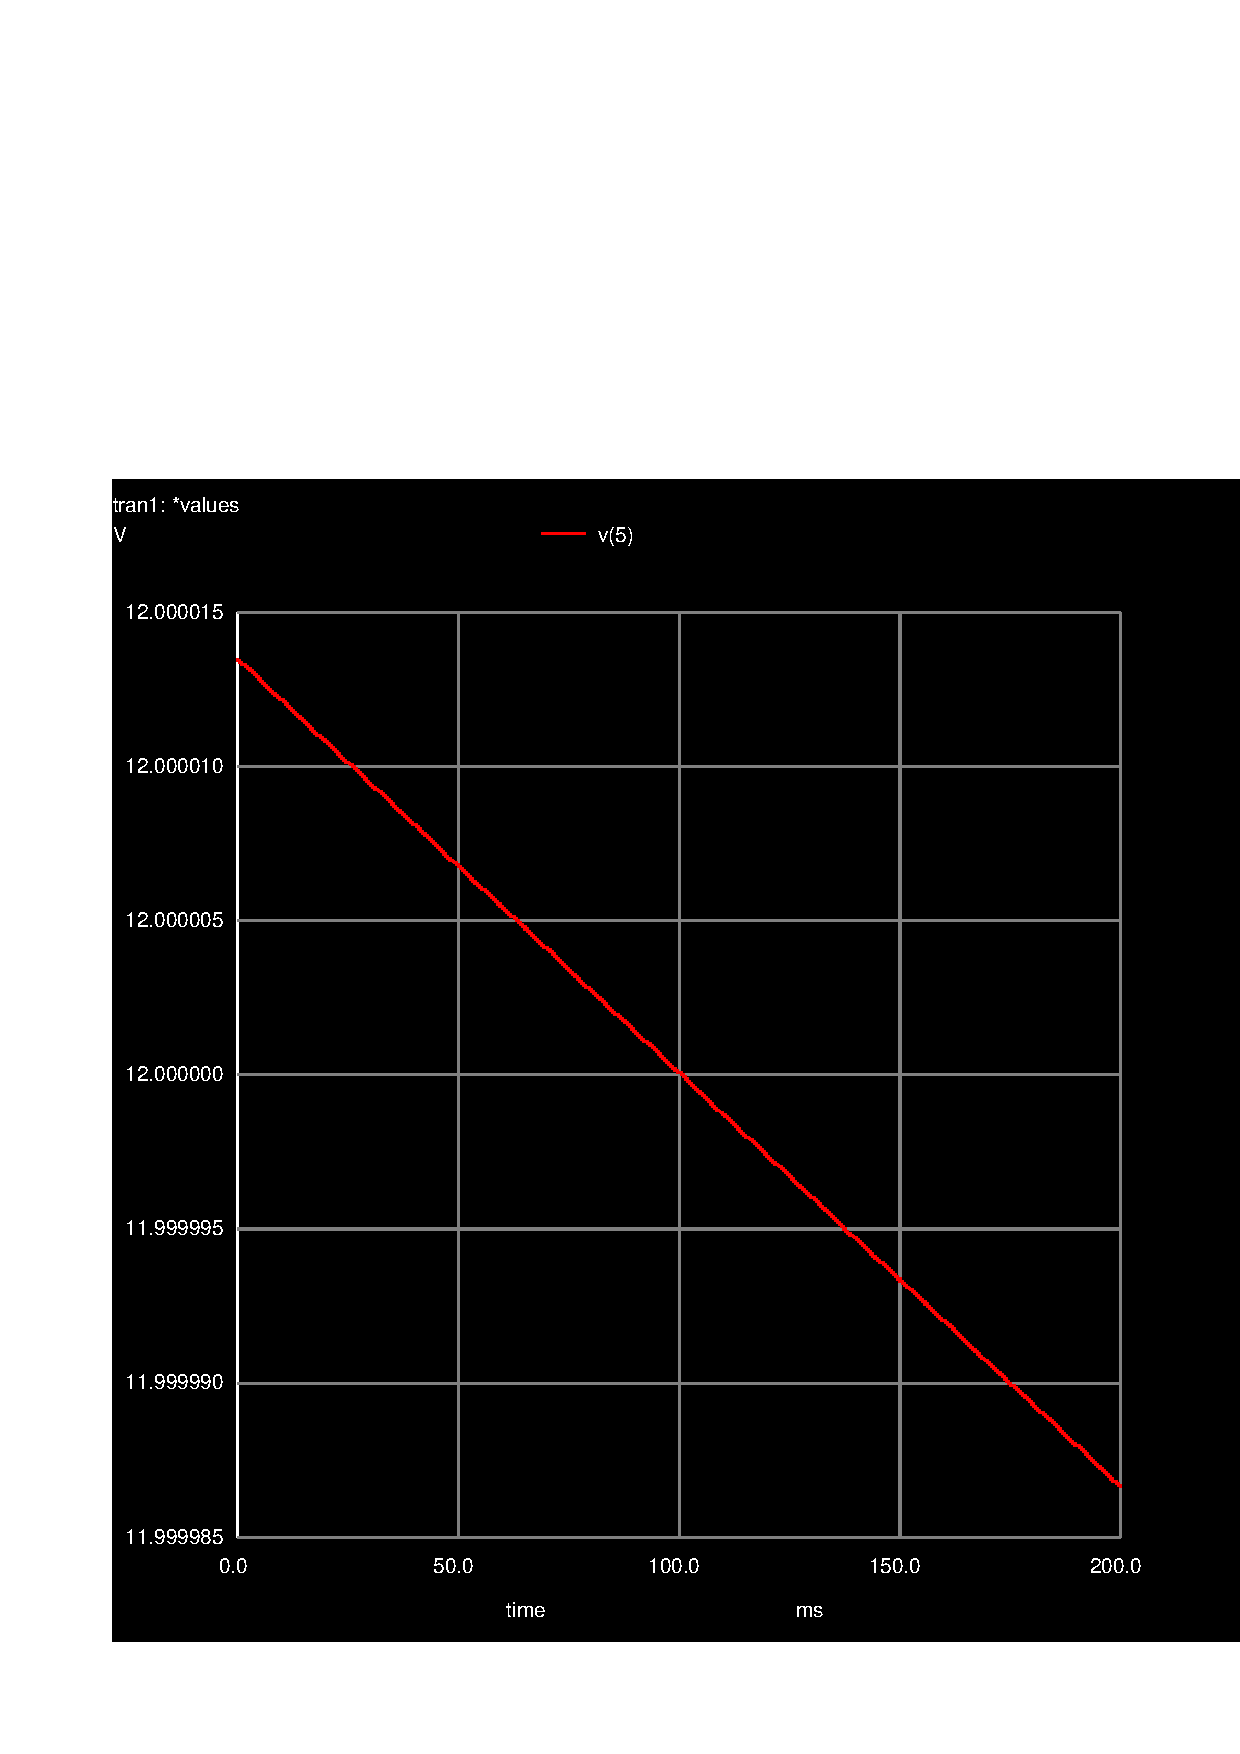
\includegraphics[width=0.5\linewidth]{vout.pdf}
\caption{The input and output signals, superimposed. The sheer scale of the amplification is evident here (the input, given the linear scale, is nearly a straight line with but only little ondulation around zero). The y axis is in V. Note that this graph is for the transient analysis, for which the voltage source only puts out 10mV, that with a gain of around $10^{2}$ goes to somewhere around 1V.}
\label{fig:In_imp}
\end{figure}
\vspace{-3cm}


\begin{figure}[H] \centering
\includegraphics[width=0.5\linewidth]{vp_out.pdf}
\caption{Phase bode plot of the circuit. Note how the plot decreases from plus 90 degrees down to zero, followed by a full 180 degree drop and finally another 90 degree drop, back to the initial plus 90 degrees phase. This indicates the existence of an additional two poles in the OPAMP model, not present in the ideal model we used for the theory section. If you remember the theoretical bode plot we obtained from octave, it is completely different! Note also that there is no discontinuity in this plot, it is just the way Ngspice presents the output of the arg() funtion, in the domain -180 degrees to 180 degrees.}
\label{fig:out_imp}
\end{figure}
\vspace{-3cm}


\pagebreak

\pagebreak
\section{Conclusion}
\label{sec:conclusion}

In this laboratory assignment the objective of analysing an RC circuit has been
achieved. Static, time and frequency analyses have been performed both
theoretically using the Octave maths tool and by circuit simulation using the
Ngspice tool. The simulation results matched the theoretical results
precisely. The reason for this perfect match is the fact that this is a
straightforward circuit containing only linear components, so the theoretical
and simulation models cannot differ. For more complex components, the
theoretical and simulation models could differ but this is not the case in this
work.


%\cleardoublepage

% ----------------------------------------------------------------------
%  Bibliography
% ----------------------------------------------------------------------
%\addcontentsline{toc}{section}{\bibname}
%\bibliographystyle{abbrvunsrtnat} % <<<<< SELECT IF USING REFERENCES BY NUMBER (CITATION ORDER)
%\bibliography{../../../BIBfile.bib}

% ----------------------------------------------------------------------
\end{document}
% ----------------------------------------------------------------------

